\chapter{Laplaciano sobre árboles}
\label{chapter_3}

\section{Matriz Laplaciana}
Dado un grafo simple G con $n$ vértices, definimos la matriz Laplaciana $L\in \bb{M}_n(\R)$ como :
$$ L = D-A,$$
donde $D,A$ son las matrices de grados e incidencia del grafo, respectivamente. Así, se tiene que las entradas de esta matriz estarán dadas por:
$$
L_{i, j}\coloneqq \left\{\begin{array}{ll}
\operatorname{grado}\left(v_{i}\right) & \text { si } i=j, \\
-1 & \text { si } i \neq j \text { y } v_{i} \text { es adyacente a } v_{j}, \\
0 & \text { e.o.c. }
\end{array}\right.$$
Esta matriz tiene propiedades, de las cuales nombraremos  las que nos interesan:
\begin{itemize}
	\item[$\diamond$] $L$ es simétrica;
	\item[$\diamond$] $L$ es semidefinida-positiva (sus autovalores son positivos);
	\item[$\diamond$] La suma por filas o columnas es $0$.
\end{itemize}
Esta matriz es llamada así, puesto que coincide con el laplaciano discreto. Ver por ejemplo \cite{networksAI}. Razón por la cual podemos hacer una interpretación del mismo.

\section{Operador Laplaciano discreto}
Supongamos una función $\vec{\phi}(t)$ que describe la distribución de calor dentro de un grafo en un tiempo dado. Así, $\phi_i(t)$ es el calor en el nodo $i$ en el tiempo $t$. Luego, el calor transferido entre los nodos $i$ y $j$ es directamente proporcional a la difencia de calor entre los mismos \footnote{Ley de enfriamiento de Newton}, es decir, proporcional a $\phi_i(t)-\phi_j(t)$. Así, para una constante $k$ (conocida como constante de capacidad de calor) esto se representa de la siguiente forma:

\[
\begin{aligned}
\frac{d \phi_{i}(t)}{d t} &=-k \sum_{j} A_{i j}\left(\phi_{i}(t)-\phi_{j}(t)\right) \\
&=-k\left(\phi_{i}(t) \sum_{j} A_{i j}-\sum_{j} A_{i j} \phi_{j}(t)\right) \\
&=-k\left(\phi_{i}(t) \operatorname{grado}\left(v_{i}\right)-\sum_{j} A_{i j} \phi_{j}(t)\right) \\
&=-k \sum_{j}\left(\delta_{i j} \operatorname{grado}\left(v_{i}\right)-A_{i j}\right) \phi_{j}(t) \\
&=-k \sum_{j}\left(\ell_{i j}\right) \phi_{j}(t),
\end{aligned}
\]
que se reescribe como:
\[
\begin{aligned}
\frac{d \vec{\phi}(t)}{d t} &=-k(D-A) \vec{\phi}(t) \\
&=-k L \vec{\phi}(t),
\end{aligned}
\]
es decir:
\begin{equation}\label{heateq}
\frac{d \vec{\phi}(t)}{d t}+k L \vec{\phi}(t)=0.
\end{equation}
Nótese que la ecuación \ref{heateq} tiene la forma de la ecuación de calor, donde la matriz $L$ toma el valor de $\nabla^2$. Por esta razón, hablamos de $L$ como el Laplaciano de un grafo.

Además, la ecuación \ref{heateq} es un sistema de ecuaciones de primer orden cuya solución para $\vec{\phi}(t)$ es una combinación lineal de autovectores de $L$(con autovalores $(\lambda_i)$):

$$\sum_{i=1}^{\abs{V}}c_i(t)\vec{v_i},\text{ con $V$ es el conjunto de vértices.}$$
Reemplazando en la ecuación \ref{heateq}, tenemos:

\begin{align*}
\frac{d\left(\sum_{i} c_{i}(t) \vec{v}_{i}\right)}{d t}+k L\left(\sum_{i} c_{i}(t) \vec{v}_{i}\right) &=0 \\
\sum_{i}\left[\frac{d c_{i}(t)}{d t} \vec{v}_{i}+k c_{i}(t) L \vec{v}_{i}\right] &=\\
\sum_{i}\left[\frac{d c_{i}(t)}{d t} \vec{v}_{i}+k c_{i}(t) \lambda_{i} \vec{v}_{i}\right] &;\\
\Rightarrow \frac{d c_{i}(t)}{d t}+k \lambda_{i} c_{i}(t) &=0,
\end{align*}
que es una ecuación homogénea, cuya solución está dada por:
$$c_i(t)=c_i(0)e^{-k\lambda_it}.$$
\begin{definition}[Árbol de Cayley]
	Un árbol en el cual todos sus nodos que no son hojas tiene un número constante de ramas $n$, es llamado \textit{$n$-árbol de Cayley.}
\end{definition}

\begin{center}
	\begin{figure}[h]
		\begin{tikzpicture}[x=0.75pt,y=0.75pt,yscale=-1,xscale=1]
		%uncomment if require: \path (0,300); %set diagram left start at 0, and has height of 300
		
		%Straight Lines [id:da5842217325180374] 
		\draw    (198.71,51.5) -- (199,102) ;
		%Straight Lines [id:da7276215169992284] 
		\draw    (160,140) -- (199,102) ;
		%Straight Lines [id:da28480116898973207] 
		\draw    (240,140) -- (199,102) ;
		%Straight Lines [id:da9834829913476775] 
		\draw    (312.71,100) -- (371.71,100) ;
		%Straight Lines [id:da9583545055171534] 
		\draw    (312.71,100.5) -- (290,140) ;
		%Straight Lines [id:da9799941223701523] 
		\draw    (290,59.5) -- (312.71,100.5) ;
		%Straight Lines [id:da38279622647558265] 
		\draw    (394,61.17) -- (371.71,100) ;
		%Straight Lines [id:da07459517917616099] 
		\draw    (371.71,100) -- (394,140.17) ;
		%Straight Lines [id:da3965956580664982] 
		\draw    (489,51.5) -- (489,79.5) ;
		%Straight Lines [id:da016839034481049175] 
		\draw    (472,99.17) -- (489,79.5) ;
		%Straight Lines [id:da7562850854840744] 
		\draw    (509,99.17) -- (489,79.5) ;
		%Straight Lines [id:da8034784066626488] 
		\draw    (452.67,90.17) -- (472,99.17) ;
		%Straight Lines [id:da8680080185249526] 
		\draw    (461.67,121.17) -- (472,99.17) ;
		%Straight Lines [id:da4124727277691931] 
		\draw    (509,99.17) -- (532.67,90.17) ;
		%Straight Lines [id:da2855392219619475] 
		\draw    (509,99.17) -- (519.67,123.17) ;
		
		
		
		
		\end{tikzpicture}
		\caption{3-árboles de Cayley}
	\end{figure}
\end{center}

Nótese que la definición anterior viene dada por la definición de grafo de Cayley. Además, dado que los números $p$-ádicos se pueden representar en $p$-árboles de Cayley, presentamos algunas ecuaciones.


%Nótese que $0<\omega(x,y)\leq 1$ para todo $x,y \in \Qp$.
\newpage
\subsection{Matriz de transición}
En el anterior capítulo definimos el grupo $GpnN$ (\ref{GpnN}):
\begin{equation*}
GpnN := \Big\{x\in \Qp : x = \sum_{k=-N}^{-n} a_{k} p^{k} \text{, $a_k\in \{0,\cdots,p-1\}$ y } p^{n}\leq \pnorm{x}\leq p^N\Big \}.
\end{equation*}
Nótese que $GpnN$ tiene cardinal $p^{N-n+1}$(recordemos que $n\leq0$), luego $GpnN$ es finito y así, podemos indexar sus elementos, sean $\{x_1,\dots,x_{p^{N-n}},x_{p^{N-n+1}}\}$ y corresponderlos inyectivamente con el conjunto $\{1,\dots,p^{N-n},p^{N-n+1}\}$ a través de la siguiente función:
\begin{align*}
&l\colon\{1,\dots,p^{N-n+1}\}\to GpnN \Rightarrow l(i)=x_i.
%	&l^{-1}\colon GpnN\to \{1,\dots,p^{N-n+1}\} \Rightarrow l^{-1}(x)= l^{-1}\big(\sum_{k=N}^{n}a_kp^{-k}\big)=1+p^{-1}\sum_{k=N}^{n}a_kp^k,
\end{align*}

Definimos una \textit{matriz de réplica} a la matriz $\textbf{Q   }=(Q_{ab}) $ de tamaño $p^{N-n+1}\times p^{N-n+1}$, como un operador en el espacio de funciones del conjunto $\{1,\dots,p^{N-n+1}\}$ tal que 
\begin{equation}\label{Q}
Q_{ij}=\rho(\pnorm{l(i)-l(j)}),
\end{equation}
donde $\rho$ es una función que depende de la distancia $p$-ádica entre $l(i)$ y $l(j)$. 
Luego, la estructura de la matriz $\textbf{Q}$ con $p=2$ es de tipo Parisi (\cite{Parisi-2000}):
$$
\boldsymbol{Q}=\left(\begin{array}{lllllllll}
0 & q_{1} & q_{2} & q_{2} & q_{3} & q_{3} & q_{3} & q_{3} & \dots \\
q_{1} & 0 & q_{2} & q_{2} & q_{3} & q_{3} & q_{3} & q_{3} & \dots \\
q_{2} & q_{2} & 0 & q_{1} & q_{3} & q_{3} & q_{3} & q_{3} & \dots \\
q_{2} & q_{2} & q_{1} & 0 & q_{3} & q_{3} & q_{3} & q_{3} & \dots \\
q_{3} & q_{3} & q_{3} & q_{3} & 0 & q_{1} & q_{2} & q_{2} & \dots \\
q_{3} & q_{3} & q_{3} & q_{3} & q_{1} & 0 & q_{2} & q_{2} & \dots \\
q_{3} & q_{3} & q_{3} & q_{3} & q_{2} & q_{2} & 0 & q_{1} & \dots \\
q_{3} & q_{3} & q_{3} & q_{3} & q_{2} & q_{2} & q_{1} & 0 & \dots\\
&  &  &  & \vdots & & &  & \ddots
\end{array}\right)
$$
Luego, definimos la \textit{matriz de transición } $W$, a partir de la matriz de réplica como:
\[   
W_{ij} =
\begin{cases}
Q_{ij} & i\neq j,\\
-\sum_{\gamma \neq i}^{N-n+1}Q_{i\gamma} &i=j.\\

\end{cases}
\]

Dado $GpnN\subset \Qp$, sabemos que tiene una representación natural de $(N-n+1)$-árbol de Cayley. Para entender mejor la representación, tomemos como ejemplo a $G2\_11$; nótese que $\abs{G2\_11}=8$, por lo tanto, podemos indexar sus elementos en $\{1,\dots,8\}$, ver por ejemplo \ref{G2_11}. Luego $G2\_11$ tendrá una matriz de transición $W$ con la siguiente estructura (matriz de Parisi):

\[
W=
\left[
\begin{array}{c|c}
\begin{array}{c|c}
\begin{array}{cc}
w_0 & w_1 \\

w_1 & w_0
\end{array} & w_2 \\
\hline
w_2 & \begin{array}{cc}
w_0 & w_1 \\

w_1 & w_0
\end{array}

\end{array} & w_3 \\
\hline
w_3 & \begin{array}{c|c}
\begin{array}{cc}
w_0 & w_1 \\

w_1 & w_0
\end{array}& w_2 \\
\hline
w_2 &\begin{array}{cc}
w_0 & w_1 \\

w_1 & w_0
\end{array}
\end{array}
\end{array}
\right]
\]

\begin{figure}
	\caption{$G2\_11$}
	\label{G2_11}
	\centering
	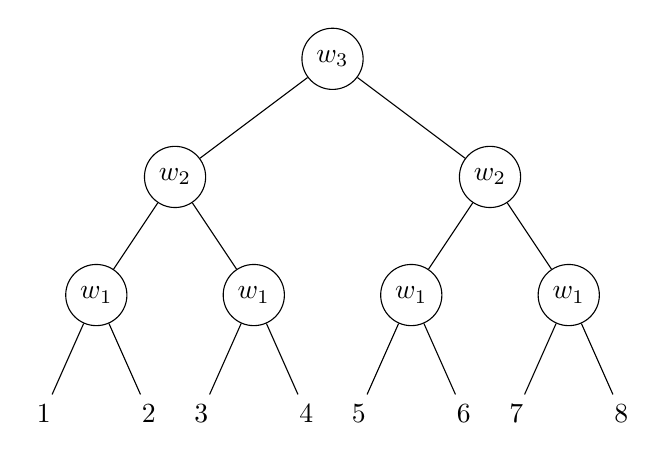
\begin{tikzpicture}[level/.style={sibling distance=40mm/#1}]
	\node [circle,draw] (z){$w_3$}
	
	child {node [circle,draw] (a) {$w_2$}
		child {node [circle,draw] (b) {$w_1$}
			child {node {$1$}}
			child {node {$2$}}
		}
		child {node [circle,draw] (g) {$w_1$}
			child {node {$3$}}
			child {node {$4$}}
		}
	}
	child {node [circle,draw] (j) {$w_2$}
		child {node [circle,draw] (k) {$w_1$}
			child {node {$5$}}
			child {node {$6$}}
		}
		child {node [circle,draw] (l) {$w_1$}
			child {node {$7$}}
			child {node {$8$}}
		}
	};
	\end{tikzpicture}%}
\end{figure}
En general, esta matriz muestra las interacciones entre los nodos hojas (que es donde inicialmente se encuentran los números $p$-ádicos en la representación dada en el capítulo anterior). Además, dado que la ecuación \ref{Q} establece que la matriz depende de la distancia asociada a dos estados $i,j\in\{1, \dots,p^{N-n+1}\}$, damos un ejemplo de tales matrices $Q_{ij}$, tomando $\rho$ como sigue:
\begin{equation}
\label{f_prob}
Q_{ij}=\rho(\pnorm{l(i)-l(j)})= \frac{C}{\pnorm{x-y}^\alpha + 1},\text{ $x,y\in GpnN$}.
\end{equation}

%y representa la tasa de transición de $x_i$ a $x_j$. La construcción de esta matriz tiene motivación en Biología, y más específicamente en el estudio de proteinas (ver \cite{Avetisov-1999,Avetisov-2002,Parisi-2000}). Siendo así, podemos definir la ecuación maestra.

\begin{figure}
	\begin{subfigure}{.6\textwidth}
		\centering
		\includegraphics[width=.8\linewidth]{img/matrix/matrixG2_22}
		\caption{Matriz de $\mathit{G2\_22}$}
		\label{fig:sfig1}
	\end{subfigure}%
	\begin{subfigure}{.6\textwidth}
		\centering
		\includegraphics[width=.8\linewidth]{img/matrix/matrixG2_32}
		\caption{Matriz de $\mathit{G2\_32}$}
		\label{fig:sfig2}
	\end{subfigure}
	\begin{subfigure}{.6\textwidth}
		\centering
		\includegraphics[width=.8\linewidth]{img/matrix/matrixG2_33}
		\caption{Matriz de $\mathit{G2\_33}$}
		\label{fig:sfig1}
	\end{subfigure}%
	\begin{subfigure}{.6\textwidth}
		\centering
		\includegraphics[width=.8\linewidth]{img/matrix/matrixG2_43}
		\caption{Matriz de $\mathit{G2\_43}$}
		\label{fig:sfig1}
	\end{subfigure}%
	
	\caption{Matrices de Parisi asociadas a los estados de las figuras \ref{2adics_trees} con $\alpha=2$ y $C=3$}
	\label{2adic_matrices}
\end{figure}
\pagebreak

\subsection{Ecuación de ultradifusión}
Análogamente a como se estableció la ecuación de calor sobre grafos(\ref{heateq}), definimos la ecuación maestra como sigue:
\begin{equation}
\label{ME}
\frac{du_i(t)}{dt} = \sum_{j\neq i}W_{ji}u_j(t) - \sum_{j\neq i}W_{ij}u_i(t), 
\end{equation}
donde $u_i$ es la probabilidad de transición, es decir, la probabilidad de pasar del estado $i$ al estado $j$ en el tiempo $t$.

Además, como hicimos con la ecuación \ref{heateq}, podemos llevar la ecuación \ref{ME} a la forma:
$$\frac{du(t)}{dt} = Wu(t).$$
Cuya solución, estará dada de manera estándar como una combinación lineal de autovectores de $W$:
$$u(t)=\sum_{i=1}^{p^{N-n+1}}c_i(t)v_i.$$
Con:
$$c_i(t)=c_i(0)e^{\lambda_it}.$$

Así, la solución numérica del problema anterior con distintas condiciones iniciales está dada por las figuras \ref{IC-const}, \ref{IC-random} y \ref{IC-bell}.               

\begin{figure}
	\begin{subfigure}{.5\textwidth}
		\centering
		\includegraphics[width=.8\linewidth]{img/solutions/ones_0}
		\caption{$t=0$}
		\label{fig:sfig1}
	\end{subfigure}%
	\begin{subfigure}{.5\textwidth}
		\centering
		\includegraphics[width=.8\linewidth]{img/solutions/ones_1}
		\caption{$t=3.33$}
		\label{fig:sfig1}
	\end{subfigure}
	\begin{subfigure}{.5\textwidth}
		\centering
		\includegraphics[width=.8\linewidth]{img/solutions/ones_2}
		\caption{$t=6.67$}
		\label{fig:sfig1}
	\end{subfigure}%
	\begin{subfigure}{.5\textwidth}
		\centering
		\includegraphics[width=.8\linewidth]{img/solutions/ones_3}
		\caption{$t=10$}
		\label{fig:sfig1}
	\end{subfigure}
	\begin{subfigure}{1.05\textwidth}
		\centering
		\includegraphics[width=.8\linewidth]{img/solutions/ones_bar}
		%\caption{$t=10$}
		\label{fig:sfig1}
	\end{subfigure}%
	\caption{Comportamiento de la solución en distintos $t\in[0,10]$ para la condición inicial constante $u(0)=\vec{1}$ en $\mathit{G2\_05}.$}
	\label{IC-const}
\end{figure}



\begin{figure}
	\begin{subfigure}{.5\textwidth}
		\centering
		\includegraphics[width=.8\linewidth]{img/solutions/random_0}
		\caption{$t=0$}
		\label{fig:sfig1}
	\end{subfigure}%
	\begin{subfigure}{.5\textwidth}
		\centering
		\includegraphics[width=.8\linewidth]{img/solutions/random_1}
		\caption{$t=3.33$}
		\label{fig:sfig1}
	\end{subfigure}
	\begin{subfigure}{.5\textwidth}
		\centering
		\includegraphics[width=.8\linewidth]{img/solutions/random_2}
		\caption{$t=6.67$}
		\label{fig:sfig1}
	\end{subfigure}%
	\begin{subfigure}{.5\textwidth}
		\centering
		\includegraphics[width=.8\linewidth]{img/solutions/random_3}
		\caption{$t=10$}
		\label{fig:sfig1}
	\end{subfigure}
	\begin{subfigure}{1.05\textwidth}
		\centering
		\includegraphics[width=.8\linewidth]{img/solutions/random_bar}
		%\caption{$t=10$}
		\label{fig:sfig1}
	\end{subfigure}%
	\caption{Comportamiento de la solución en distintos $t\in[0,10]$ para la condición inicial $u(0)$ aleatoriamente distribuida, con cada entrada en $[0,1]$, en $\mathit{G2\_05}$.}
	\label{IC-random}
\end{figure}

\begin{figure}
	\begin{subfigure}{.5\textwidth}
		\centering
		\includegraphics[width=.8\linewidth]{img/solutions/normal_0}
		\caption{$t=0$}
		\label{fig:sfig1}
	\end{subfigure}%
	\begin{subfigure}{.5\textwidth}
		\centering
		\includegraphics[width=.8\linewidth]{img/solutions/normal_1}
		\caption{$t=3.33$}
		\label{fig:sfig1}
	\end{subfigure}
	\begin{subfigure}{.5\textwidth}
		\centering
		\includegraphics[width=.8\linewidth]{img/solutions/normal_2}
		\caption{$t=6.67$}
		\label{fig:sfig1}
	\end{subfigure}%
	\begin{subfigure}{.5\textwidth}
		\centering
		\includegraphics[width=.8\linewidth]{img/solutions/normal_3}
		\caption{$t=10$}
		\label{fig:sfig1}
	\end{subfigure}
	\begin{subfigure}{1.05\textwidth}
		\centering
		\includegraphics[width=.8\linewidth]{img/solutions/normal_bar}
		%\caption{$t=10$}
		\label{fig:sfig1}
	\end{subfigure}%
	\caption{Comportamiento de la solución en distintos $t\in[0,10]$ para la condición inicial $u(0)$ en forma de campana de Gauss, en $\mathit{G2\_33}$.}
	\label{IC-bell}
\end{figure}